\documentclass[12pt]{article}
\usepackage{hyperref}
\usepackage{authblk}
% Document Layout
\usepackage{natbib}
\bibliographystyle{aer}

\usepackage{geometry} % Customize document dimensions, margins, and page size.
\usepackage{fancyhdr} % Extensive control of page headers and footers.
\usepackage{titlesec} % Control over section and chapter headings.

% Font and Text
\usepackage[utf8]{inputenc} % Allows input of international characters.
\usepackage[T1]{fontenc} % Font encoding.
\usepackage[english]{babel} % Multilingual support.
\usepackage{amsmath, amsfonts, amssymb} % American Mathematical Society packages for advanced math typesetting.
\usepackage{mathptmx} % Times font
\usepackage{helvet} % Helvetica font
\usepackage{courier} % Courier font

% Graphics and Tables
\usepackage{graphicx} % Enhanced support for graphics.
\usepackage{subfigure} % or use \usepackage{subcaption} for handling sub-figures within a single figure environment.
\usepackage{float} % Improved interface for floating objects (tables, figures).
\usepackage{wrapfig} % Allows figures or tables to have text wrapped around them.
\usepackage{pgf, tikz} % Creating high-quality diagrams and figures.
\usepackage{xcolor} % Easy driver-independent access to several kinds of color tints, shades, tones, and mixes of arbitrary colors.
\usepackage{color} 
\usepackage{tabularx} % Enhanced tables.
\usepackage{booktabs} % Publication quality tables in LaTeX.

\usepackage{threeparttable}
\usepackage{longtable}
\usepackage{pdflscape}

% Set the page size and margins
\geometry{letterpaper, portrait, margin=1in}


\title{Sketch for the Conceptual Framework}
\author[1]{Zhiyao (Yao) Ma}
\affil[1]{UC Davis}
\date{\today}


\begin{document}
\maketitle
\tableofcontents
\newpage


\section{Two-Period Storage Model with Buyer Competition}

In many agricultural contexts, farmers must decide whether to sell their harvested crop immediately or store it for a future sales period, with storage often incurring an opportunity cost or physical cost. Farm-gate prices may differ across periods due to time-varying market competitive conditions even under a stable downstream demand.

This theoretical framework focuses on how the farmer uses storage as a strategic tool in response to inter-temporal buyer competitiveness changes and how their storage decisions vary across other parameters, like risk aversion and composite storage cost.

\subsection{Interpreting the Storage Decision \boldmath{\(s\)}}

Let \(s\in [0,1]\) denote how much of the harvest is allocated to the second period, then:
\[
(1-s)\,q 
\quad\text{is sold in period 1, and}\quad 
s\,q 
\quad\text{is sold in period 2.}
\]
Alternatively, if the farmer (or each farmer in a population) can only choose \emph{all-or-nothing} storage, then \(s\) can be seen as the probability (or fraction of farmers) adopting the ``store'' strategy. In expectation, both interpretations yield the same mathematical form.

\subsection{Model Setup}

\begin{itemize}
    \item \(q\): Total harvest (fixed).
    \item \(p_1\): First-period price (observed, deterministic).
    \item \(p_2\): Second-period price (random).
    \item \(\theta\): Buyer-competition intensity in period~2. A larger \(\theta\) implies a higher distribution of \(p_2\).
    \item \(\delta \in (0,1]\): Discount/storage factor (closer to 1 means cheaper storage or more patience).
    \item \(\gamma\): CRRA parameter; typically \(0< \gamma \le 1\) for risk aversion or \(\gamma<0\) for slight risk-loving.
\end{itemize}

Period-1 revenue: \((1-s)\,q\,p_1\). 
Period-2 revenue: \(s\,q\,p_2\). 
We model a CRRA utility function:
\[
U(x) 
\;=\; 
\frac{x^{\,1-\gamma}}{\,1-\gamma\,},
\]
with \(\gamma \neq 1\). (When \(\gamma=1\), this becomes \(\ln x\).) For \(\gamma>0\), \(U\) is strictly concave (risk-averse). For \(\gamma<0\), \(U\) is convex (risk-loving).

The farmer's problem is:
\[
\max_{\,0 \,\le s \,\le 1\,}
\Bigl\{
U\bigl((1-s)\,q\,p_1\bigr)
\;+\;
\delta\,\mathbb{E}_\theta\bigl[\,U(s\,q\,p_2)\bigr]
\Bigr\}.
\]
By factoring out constants (like \(q^{\,1-\gamma}\)), the objective function reduces to
\[
\max_{\,0 \le s \le 1\,}
(1-s)^{\,1-\gamma}\,p_1^{\,1-\gamma}
\;+\;
\delta\,s^{\,1-\gamma}\,\mathbb{E}_\theta\bigl[p_2^{\,1-\gamma}\bigr].
\]

\subsection{Solving the Farmer's Problem}

\subsubsection{Case 1: \(\gamma>0\) (Risk-Averse) \quad Usually \boldmath{\(\gamma \le 1\)}}

Here, \((1-s)^{1-\gamma}\) and \(s^{1-\gamma}\) are concave in \(s\). Their sum is thus concave, ensuring a standard \emph{interior} solution (unless parameters push us to the boundary). The first-order condition for an interior optimum \(0<s<1\) is:
\[
-(1-\gamma)\,(1-s)^{-\gamma}\,p_1^{\,1-\gamma}
\;+\;
\delta\,(1-\gamma)\,s^{-\gamma}\,\mathbb{E}_\theta\bigl[p_2^{\,1-\gamma}\bigr]
\;=\;0.
\]
Divide by \((1-\gamma)\):
\[
(1-s)^{-\gamma}\,p_1^{\,1-\gamma}
\;=\;
\delta\,s^{-\gamma}\,\mathbb{E}_\theta\bigl[p_2^{\,1-\gamma}\bigr].
\]
Rearrange:
\[
\left(\frac{s}{\,1-s\,}\right)^{\!\gamma}
\;=\;
\frac{\delta\,\mathbb{E}_\theta[p_2^{\,1-\gamma}]}{\,p_1^{\,1-\gamma}\,}
\;=:\;\kappa(\theta).
\]
Then the solution is
\[
s^*(\theta)
\;=\;
\frac{\kappa(\theta)^{\,1/\gamma}}
     {\,1 + \kappa(\theta)^{\,1/\gamma}\,},
\quad\text{where}\quad
\kappa(\theta)
\;=\;
\frac{\delta\;\mathbb{E}_\theta\bigl[p_2^{\,1-\gamma}\bigr]}{p_1^{\,1-\gamma}}.
\]
Because \(f(s)\) is strictly concave for \(\gamma>0\), this critical point is a global maximum \emph{unless} it ``pushes'' outside \([0,1]\). In extreme cases:
\[
\kappa(\theta)\to 0 \;\Longrightarrow\; s^*\to 0,
\quad
\kappa(\theta)\to \infty \;\Longrightarrow\; s^*\to 1.
\]
Hence, if \(\delta\) or \(\mathbb{E}_\theta[p_2^{1-\gamma}]\) are extremely large (and \(p_1\) small), we get $s^*\approx 1$; if they are very small, we get $s^*\approx 0$. However, these extreme cases are nearly impossible in most agricultural supply chains. 

\subsubsection{Case 2: \(\gamma<0\) (Slight Risk-Loving)}

If \(\gamma<0\), then \((1-\gamma)>1\) and the function \((1-s)^{1-\gamma} + s^{1-\gamma}\) is \emph{convex} in \(s\). Any stationary point in \((0,1)\) would be a \emph{minimum}, not a maximum. The global maximum then lies at a boundary: either $s=0$ or $s=1$. Specifically, the farmer compares:
\[
f(0)\;=\;p_1^{\,1-\gamma}
\quad\text{vs.}\quad
f(1)\;=\;\delta\,\mathbb{E}_\theta\bigl[p_2^{\,1-\gamma}\bigr].
\]
\begin{itemize}
    \item If $p_1^{\,1-\gamma} > \delta\,\mathbb{E}_\theta[p_2^{\,1-\gamma}]$, then $s^*=0$ (sell all now).
    \item Otherwise, $s^*=1$ (store all for the second period).
\end{itemize}

Although negative \(\gamma\) is less common in practice, it can occur if farmers exhibit risk-loving behavior. Even if $\gamma$ is only ``slightly'' negative, the curvature is enough to make partial storage suboptimal. 

\subsection{Comparative Statics}

Below, we focus on the \(0 < \gamma \le 1\) range relevant to typical smallholder contexts. We also keep in mind that if $\gamma<0$, we jump to a corner.

\paragraph{Discount Factor \boldmath{$\delta$}.}
Since $\kappa(\theta)$ is directly proportional to $\delta$, an increase in $\delta$ raises $\kappa(\theta)$. For $\gamma>0$, that shifts $s^*(\theta)$ \emph{up}, meaning the farmer stores more when storage is less costly or they are more patient. If $\gamma<0$, a higher $\delta$, a lower storage cost, makes the ``storing all'' corner more likely to dominate.

\paragraph{First-Period Price \boldmath{$p_1$}.}
In $\kappa(\theta)$, $p_1^{\,1-\gamma}$ appears in the denominator:
\[
\kappa(\theta) 
\;=\; 
\frac{\delta\,\mathbb{E}_\theta[p_2^{\,1-\gamma}]}{\,p_1^{\,1-\gamma}\,}.
\]
If $0<\gamma<1$, then $1-\gamma>0$ and an increase in $p_1$ makes $p_1^{\,1-\gamma}$ \emph{larger}, so $\kappa(\theta)$ \emph{falls} and $s^*(\theta)$ decreases. Thus, a higher $p_1$ leads the risk-averse farmer to sell more immediately. If $\gamma<0$, we revert to comparing $p_1^{1-\gamma}$ vs.\ $\delta\,\mathbb{E}[p_2^{\,1-\gamma}]$; a bigger $p_1$ can quickly tip the balance to the $s=0$ corner.

\paragraph{Second-Period Price Environment and \boldmath{$\theta$}.}
An improvement in the distribution of $p_2$ means $\mathbb{E}_\theta[p_2^{\,1-\gamma}]$ rises. That raises $\kappa(\theta)$, pushing $s^*(\theta)$ up for risk-averse farmers. For negative $\gamma$, it becomes more likely that the $s=1$ corner dominates. We specifically let $\theta$ capture buyer competition: a higher $\theta$ implies more intense bidding, boosting future prices in expectation. Thus, as $\theta$ grows, storing becomes more attractive, raising $s^*$ (for $\gamma>0$) or nudging the farmer toward $s=1$ (for $\gamma<0$).


\subsection{Numerical Illustration}

To illustrate our model clearly, let's assume prices are fixed at $p_1=6$ and expected future price $p_2=8$. I first analyze how the optimal share stored ($s^*$) varies with the risk aversion parameter $\gamma$ when $\delta=0.95$ (small storage cost), and then show how $s^*$ changes as the discount factor $\delta$ varies for different risk aversion levels.

\subsubsection{Impact of Risk Aversion on Storage Decision}

Figure~\ref{fig:gamma} depicts how the optimal storage share ($s^*$) depends on the risk aversion parameter ($\gamma$). When $\gamma$ increases, farmers become more risk-averse. Given our parameters, more risk-averse farmers tend to store less to secure immediate certain income, avoiding exposure to future price uncertainty. When $\gamma$ is negative (slightly risk-loving), the model suggests a corner solution: farmers either store all or nothing, depending on expected returns.

\begin{figure}[H]
    \centering
    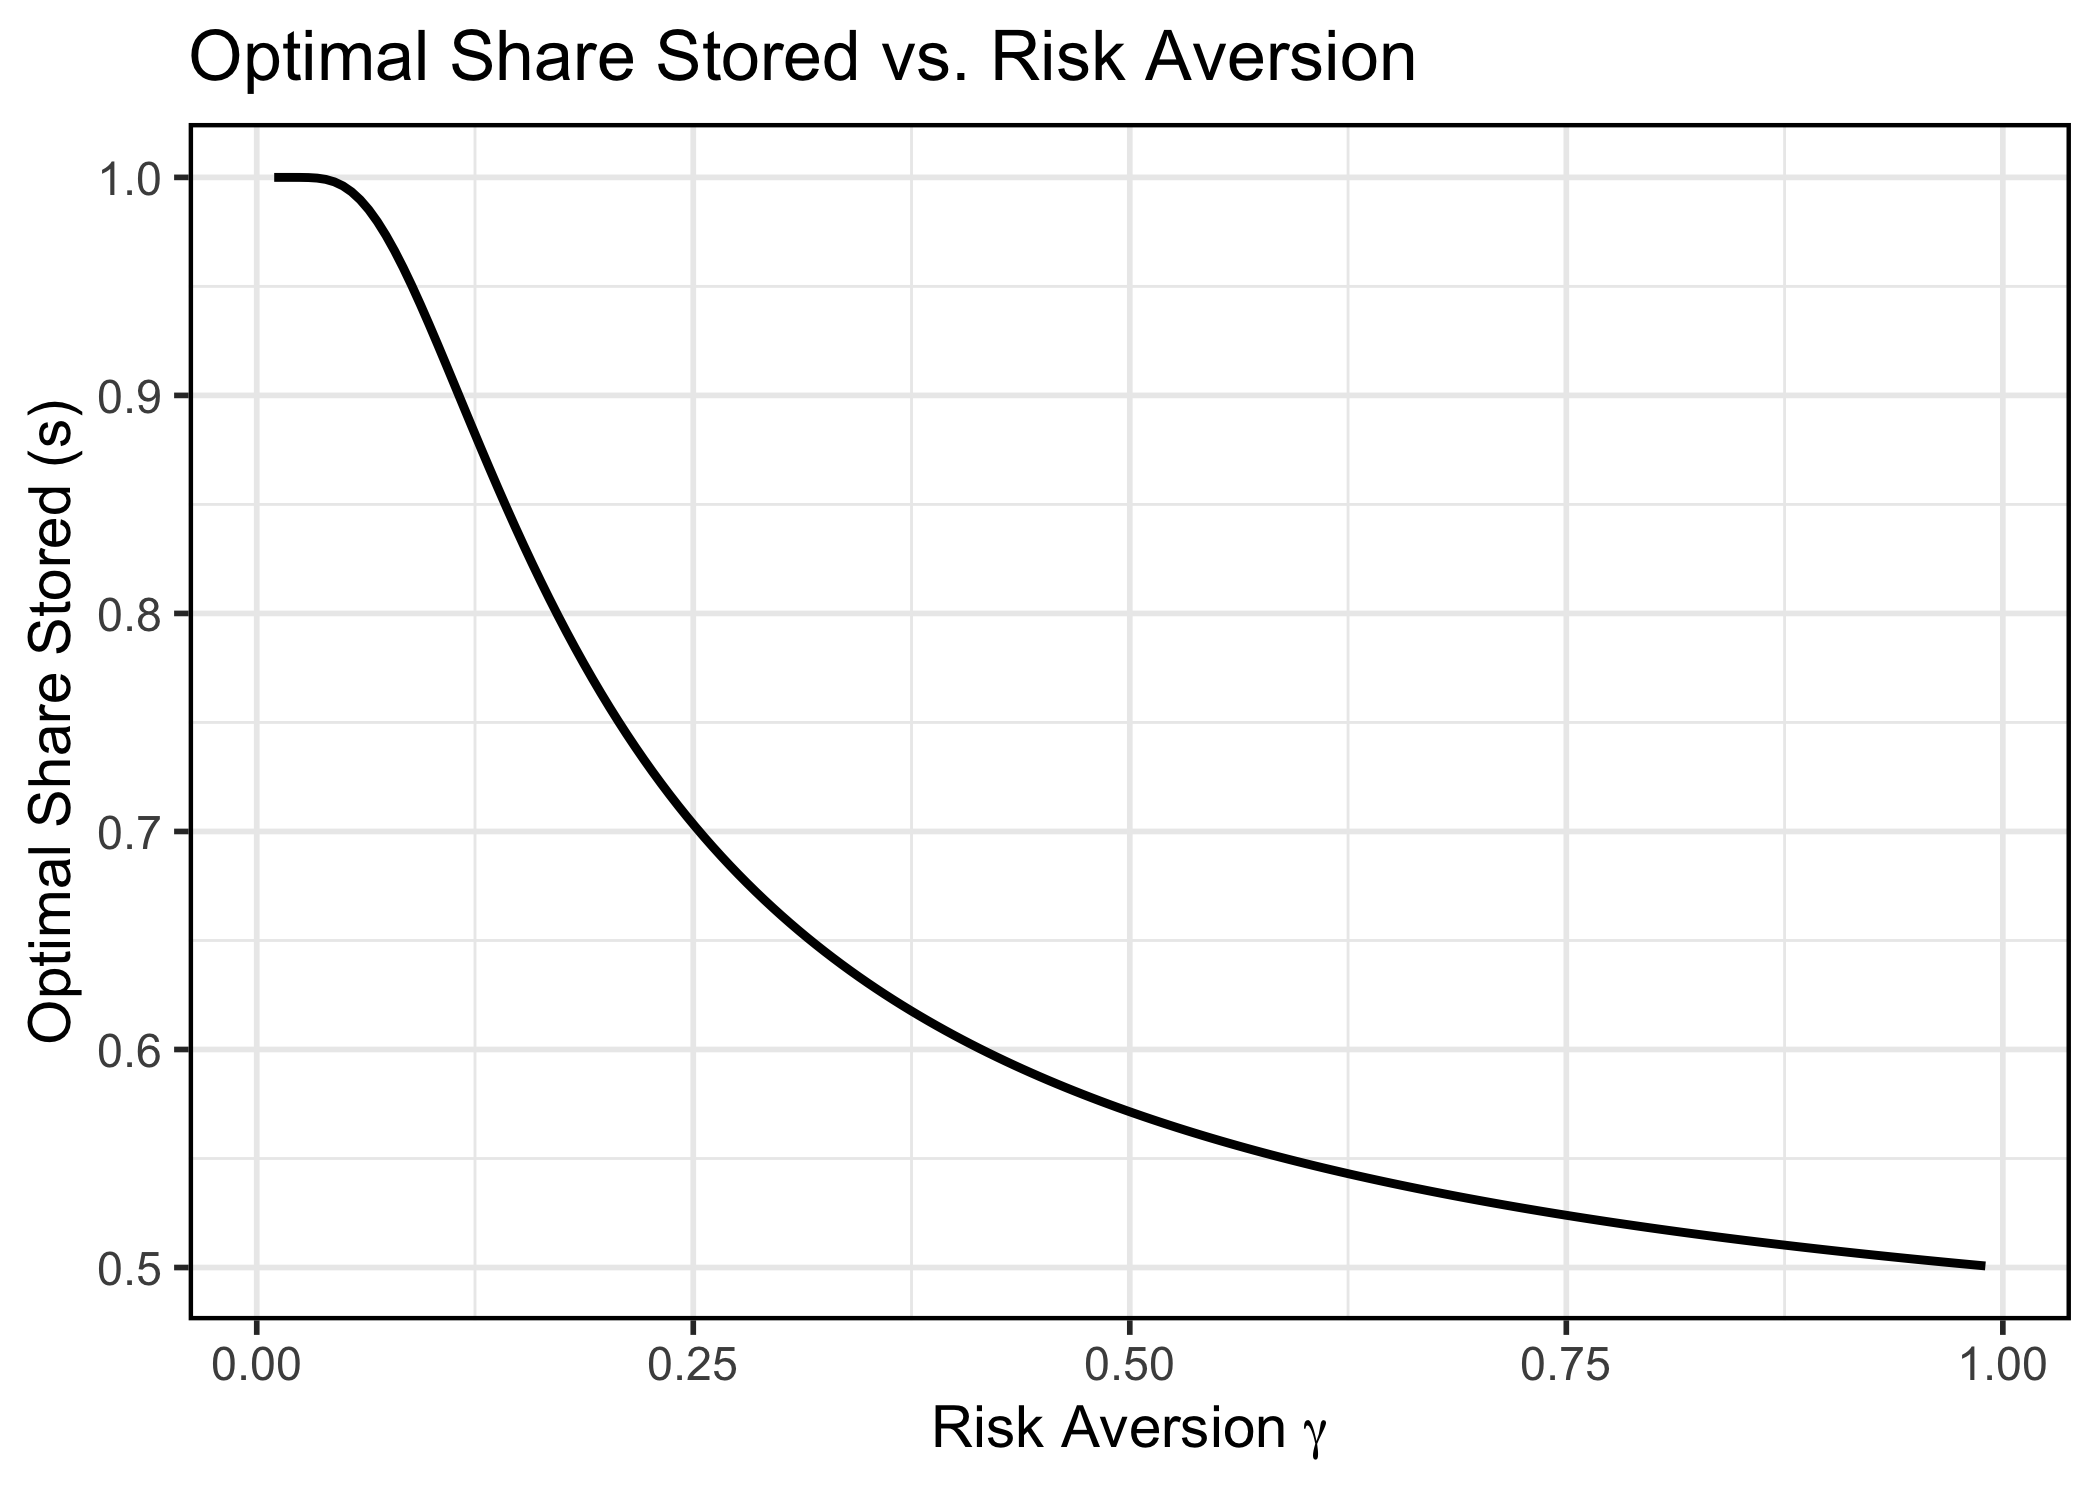
\includegraphics[width=0.75\textwidth]{s_vs_gamma.png}
    \caption{Optimal share of harvest stored ($s^*$) as risk aversion parameter ($\gamma$) varies, with $p_1=6$, $\mathbb{E}[p_2]=8$, and $\delta=0.95$. A higher $\gamma$ indicates greater risk aversion.}
    \label{fig:gamma}
\end{figure}

\textbf{Key insights:}
\begin{itemize}
    \item For $0<\gamma\leq1$, as risk aversion rises, farmers store less due to uncertainty avoidance.
    \item If $\gamma$ becomes negative (risk-loving), optimal solutions shift abruptly to corner solutions: farmers adopt a strategy of complete storage or immediate sale, driven purely by expected returns.
\end{itemize}

\subsubsection{Impact of Discount Factor on Storage Decision}

Figure~\ref{fig:delta} explores how variations in the discount factor ($\delta$) impact the storage decision under three different risk aversion levels: low ($\gamma=0.1$), moderate ($\gamma=0.3$), and high ($\gamma=0.8$).

\begin{figure}[H]
    \centering
    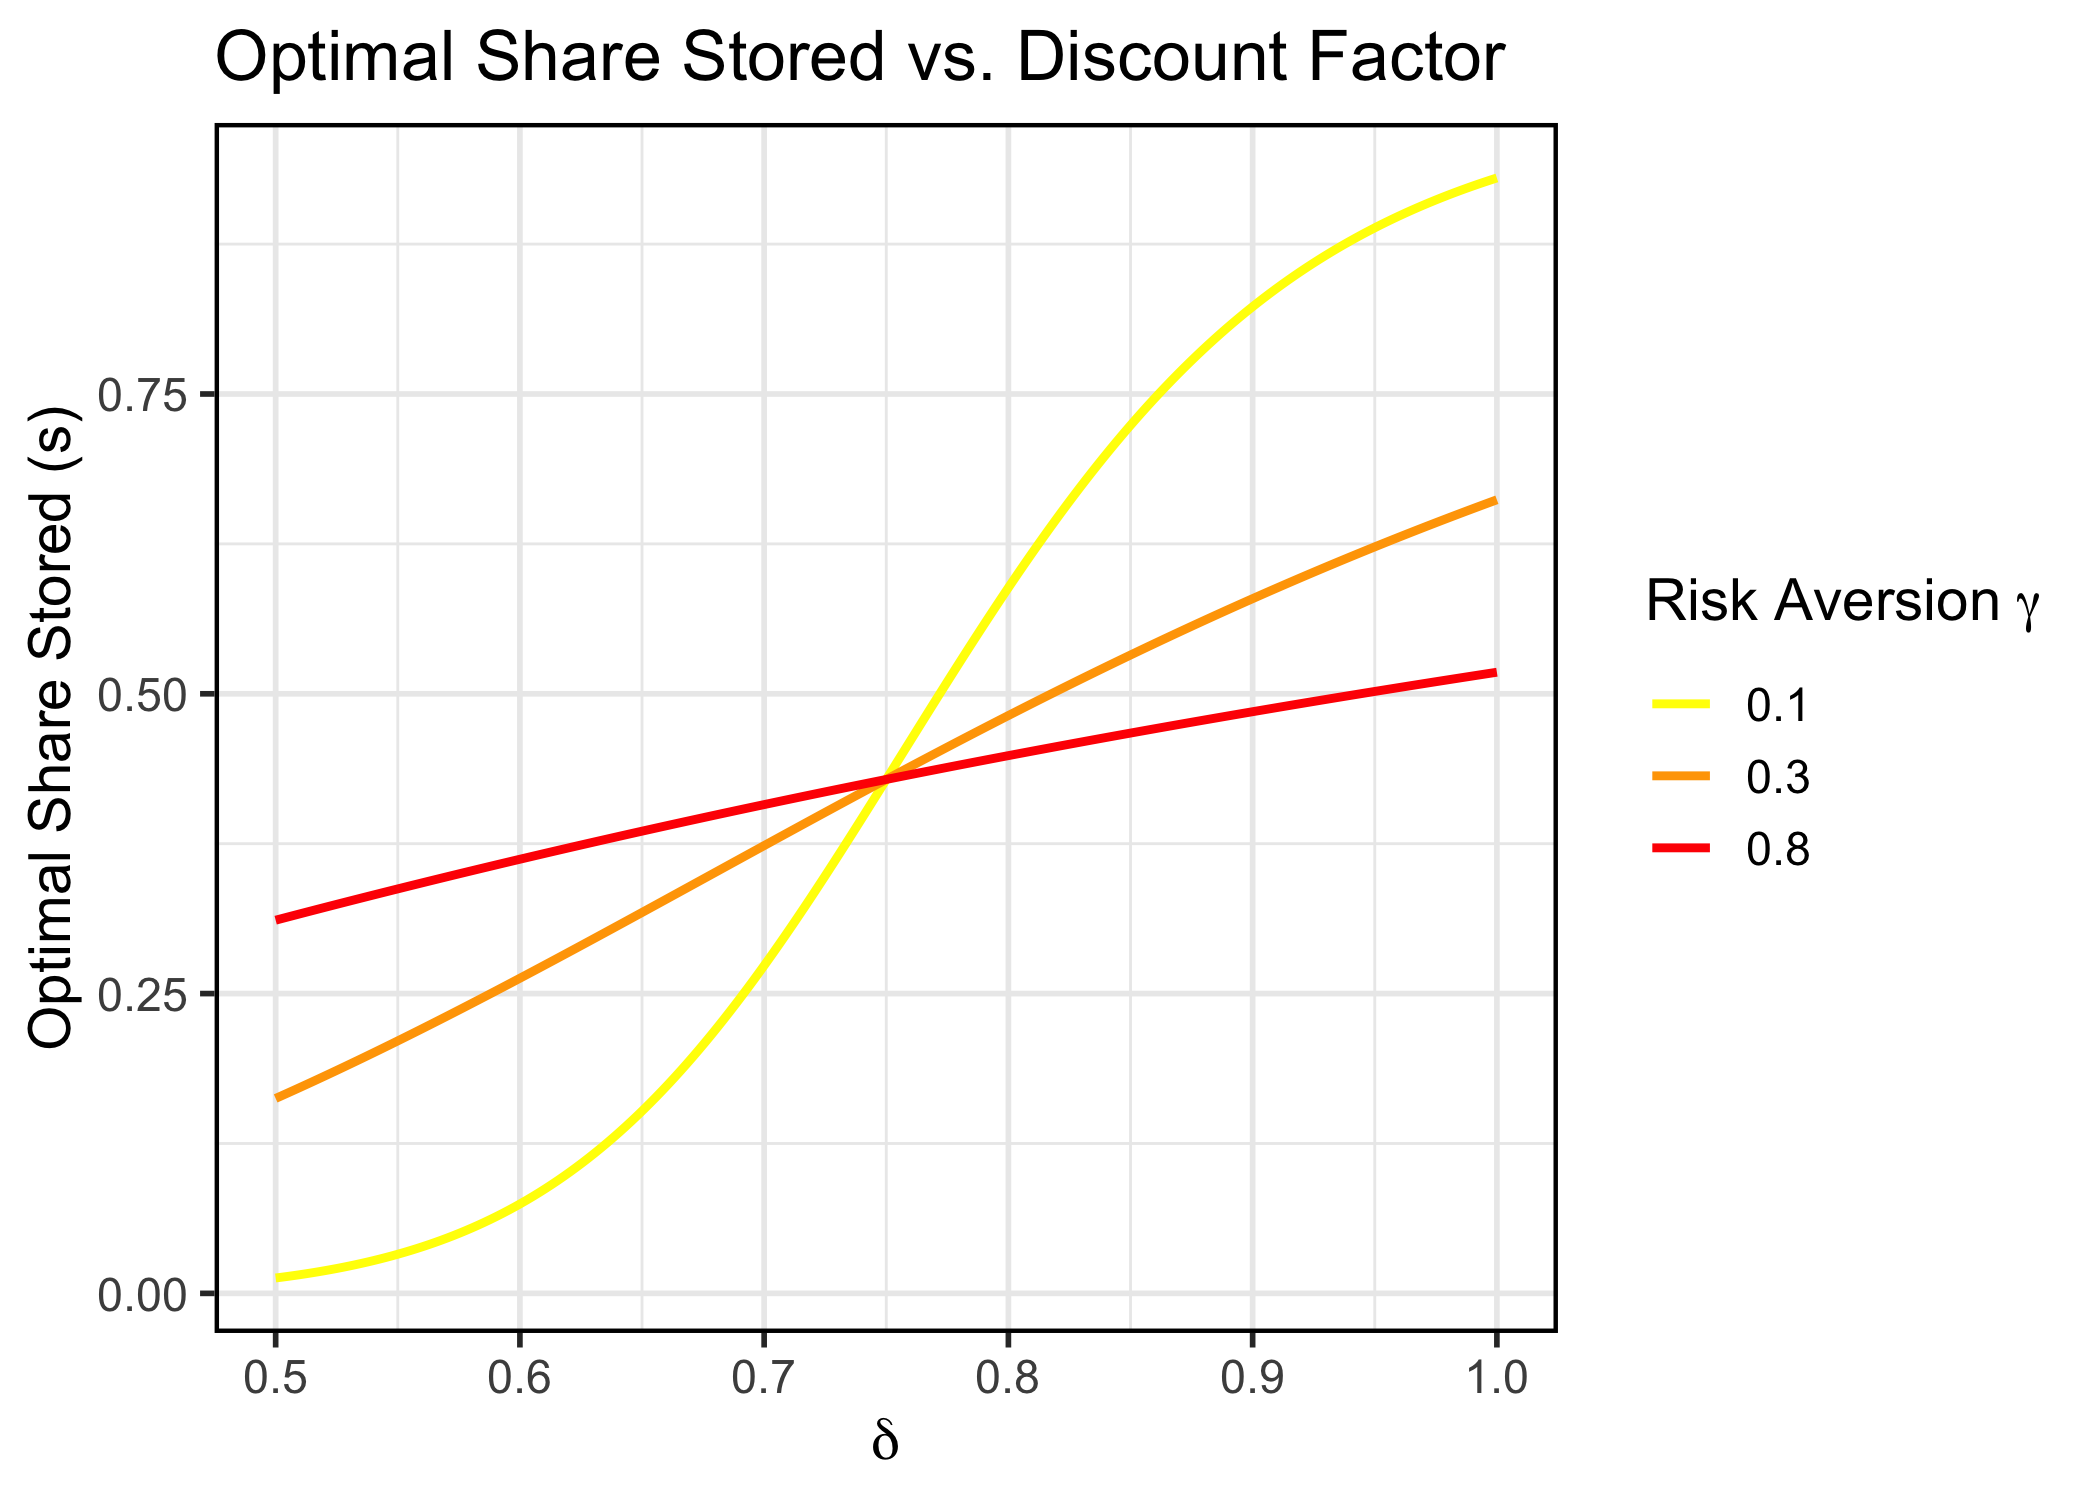
\includegraphics[width=0.75\textwidth]{s_vs_delta.png}
    \caption{Optimal share of harvest stored ($s^*$) as the discount factor ($\delta$) varies from 0 (high storage cost/impatience) to 1 (no additional storage cost). Three curves represent different risk aversion levels: low ($\gamma=0.1$, yellow), moderate ($\gamma=0.3$, orange), and high ($\gamma=0.8$, red).}
    \label{fig:delta}
\end{figure}

\textbf{Detailed observations:}
\begin{itemize}
    \item As the discount factor ($\delta$) increases, storage becomes less costly (or farmers become more patient), raising the incentive to store for future sales. Consequently, the optimal stored share ($s^*$) consistently increases.
    \item Comparing different risk aversion levels, the lowest risk aversion curve ($\gamma=0.1$, yellow) lies above the more risk-averse ones. Less risk-averse farmers store more since they are more comfortable bearing future price uncertainty.
    \item Conversely, highly risk-averse farmers ($\gamma=0.8$, red) prefer immediate and certain income. Thus, they store less overall, and their stored share only substantially increases at high discount factors (low storage costs).
\end{itemize}

\subsubsection{Role of Buyer Competition ($\theta$)}

In our extended model, the parameter $\theta$ represents buyer competition intensity in period two. Increasing $\theta$ shifts the expected future price upward, enhancing incentives to store. In terms of Figure~\ref{fig:delta}, increasing buyer competition would shift all curves upward, making storage more attractive at all discount factor levels. Similarly, higher buyer competition would raise the curves in Figure~\ref{fig:gamma}, leading farmers to store a larger share at every level of risk aversion.

These numerical illustrations concretely demonstrate the complex interplay of risk preferences, storage costs, and market expectations in shaping optimal storage decisions.



\subsection{Summary}

This two-period framework illustrates how storage decisions arise from balancing immediate versus (discounted) future revenues under uncertainty in market competitive conditions.  
\begin{itemize}
    \item If $0<\gamma\le1$ (standard risk aversion for smallholders), typically one finds an \emph{interior} solution $s^*(\theta)$ unless parameters are extreme---in which case $s^*$ might approach 0 or 1 as the best corner. 
    \item If $\gamma<0$ (mild risk-loving), the farmer goes to an \emph{all-or-nothing} corner: either sell immediately or store everything, depending on which expected payoff is larger.
    \item Strong buyer competition ($\theta$ high) elevates second-period prices, causing $s^*$ to increase (or favoring the $s=1$ corner under slight risk-loving). 
    \item A higher discount factor $\delta$ also raises $s^*$ by lowering the effective cost of waiting.
    \item A higher first-period price $p_1$ typically \emph{reduces} $s^*$ when $0<\gamma<1$, aligning with the intuition that farmers sell more now if the current price is very good.
\end{itemize}



\subsection{Graphical Analysis}

\begin{figure}[h]
    \centering
    \subfigure[Optimal Share Stored vs. Risk Aversion Parameter]{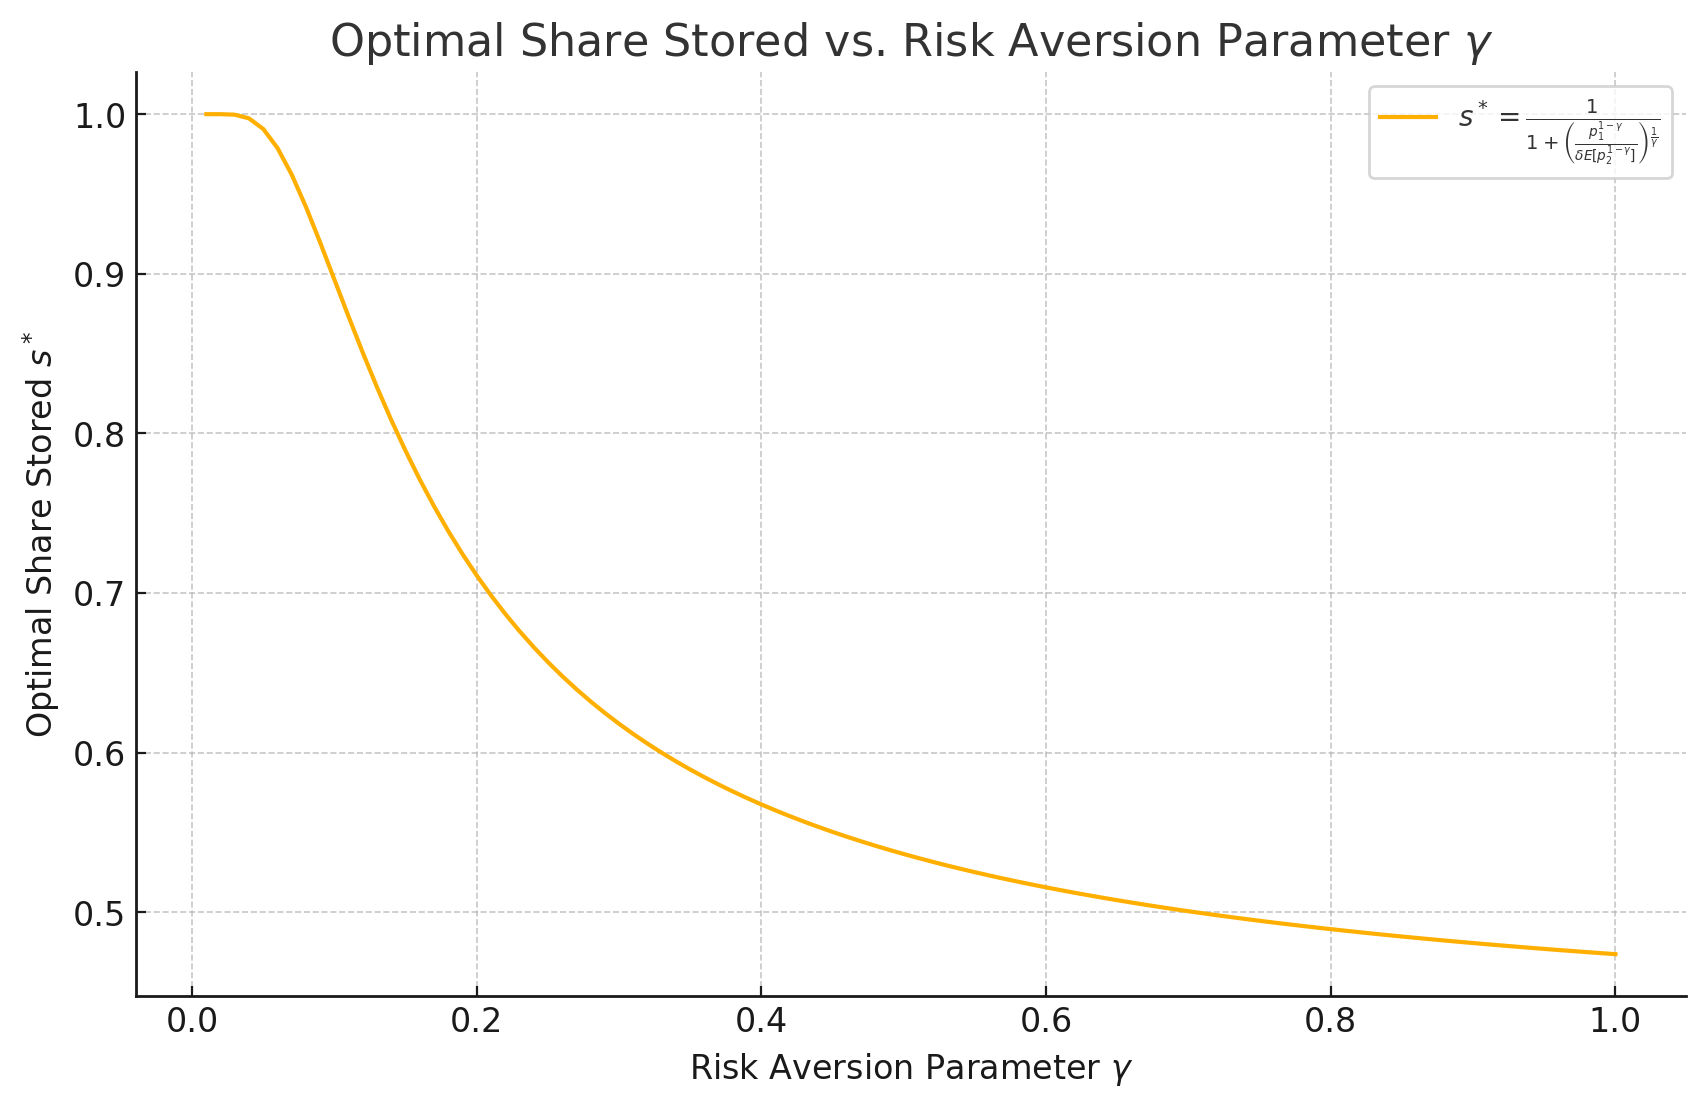
\includegraphics[width=0.45\textwidth]{figures/optimal_s_and_risk_Aversion.png}\label{fig:first}}
    \hfill
    \subfigure[Discount Factor for Different Risk Aversion Levels]{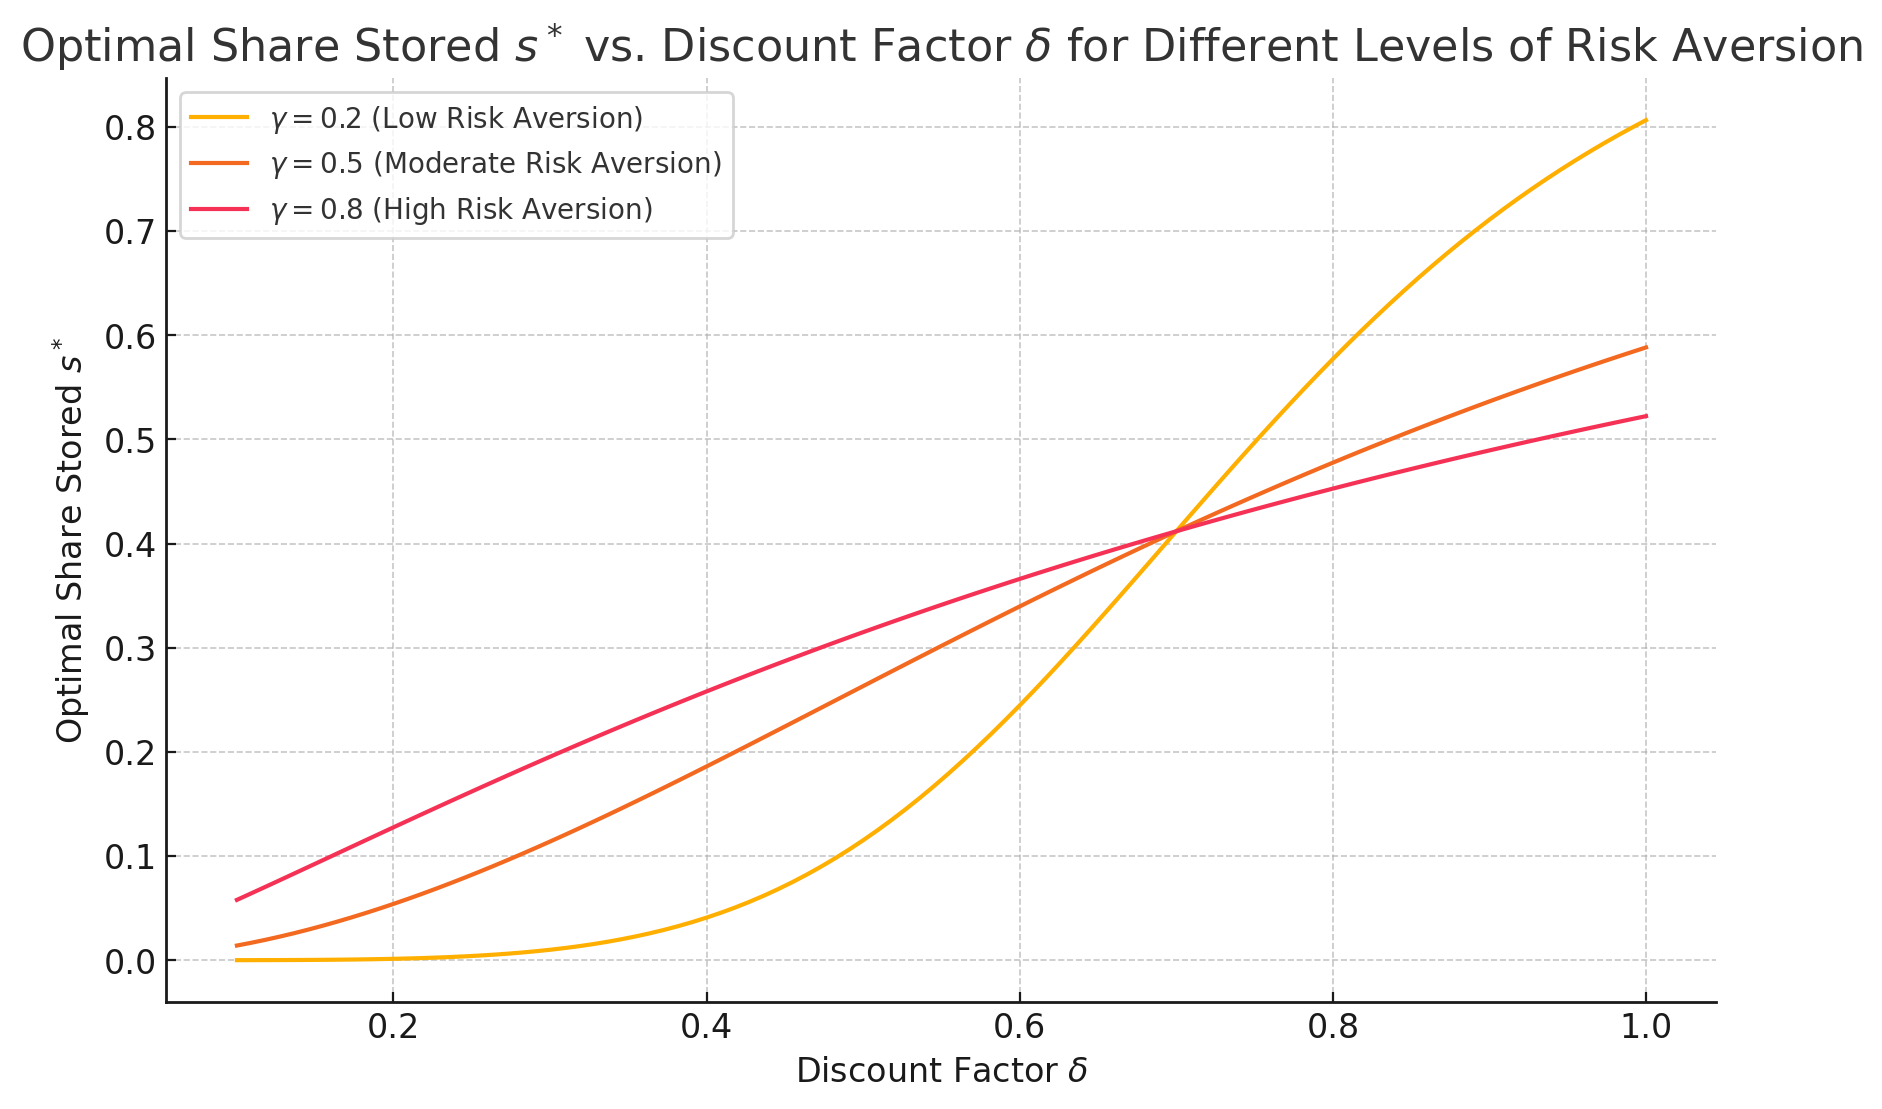
\includegraphics[width=0.45\textwidth]{figures/optimal_s_and_discount_factor.png}\label{fig:second}}
    \caption{The Movement of Optimal $s$}
    \label{fig:model demonstration}
\end{figure}


The left graph below illustrates how the optimal share of the harvest stored (\( s \)) varies with the risk aversion parameter (\( \gamma \)). In this scenario, the first-period price (\( p_1 \)) is held constant at 7, and the expected second-period price (\( E[p_2] \)) is held constant at 10. The horizontal axis represents the risk aversion parameter (\( \gamma \)), while the vertical axis shows the optimal share stored (\( s \)).

As depicted, when the farmer is less risk-averse (lower \( \gamma \)), the optimal storage share tends to be higher. Conversely, as the risk aversion increases (higher \( \gamma \)), the optimal storage share decreases. This relationship highlights that risk-averse farmers prefer to sell more in the first period when they are more concerned about future uncertainties in terms of market competition.


Keeping the prices constant at the same values, the right graph explores the impact of varying the discount factor (\( \delta \)) on the optimal storage decision. This graph features three curves, each representing different levels of risk aversion: low-risk aversion (\( \gamma = 0.2 \) in yellow), moderate risk aversion (\( \gamma = 0.5 \) in orange), and high-risk aversion (\( \gamma = 0.8 \) in red).

As the discount factor increases (storage cost gets lower), the optimal storage share also increases across all levels of risk aversion. This behavior is consistent across all risk aversion levels, though the degree of sensitivity to the discount factor varies. Farmers with lower risk aversion tend to store more as \(\delta\) increases compared to those with moderate and higher risk aversion.


According to \cite{jin2024losses}, whose fieldwork areas are highly overlapped with ours, their risk experiment indicates that the sampled apple growers are generally risk-averse, suggesting a degree of risk aversion close to the CRRA interval [0.437, 0.575). 

\cite{jin2017farmers} obtain information about subjects’ degree of relative risk aversion by assuming that individuals have a constant relative risk aversion utility function, where $r$ is the coefficient of relative risk aversion (CRRA), and $x$ is the payoff in the option. Under this specification, a CRRA coefficient $r > 0$ implies risk aversion, $r = 0$ risk neutrality, and $r < 0$ risk-seeking preferences. Column 5 in Figure \ref{fig:Risk Aversion Experiment Chart} provides the implied CRRA ranges.





% ------------------------------------------ %
% ------------------------------------------ %
% ------------------------------------------ %
\newpage
\section{Traders' Competition: Oligopsonistic Maximization Problem (Cournot)}

To capture the element of time-varying buyer-side competition and incorporate it into the price parameters in the model above, I am considering the Cournot market structure for each trading period from the traders' perspective as follows. 

\subsection{Objective and Profit Function}
In each trading period, each buyer \( i \) aims to maximize their profit \( \pi_i \). The profit for buyer \( i \) is given by:
\begin{equation}
\pi_i = r_i(q_i) - p(Q) q_i
\end{equation}
where:
\begin{itemize}
  \item \( r_i(q_i) \) is the revenue obtained from selling the purchased quantity \( q_i \).
  \item \( p(Q) \) is the inverse supply function representing the price per unit when the total quantity \( Q \) is purchased.
  \item \( q_i \) is the quantity purchased by buyer \( i \).
  \item \( Q \) is the total quantity purchased by all buyers, \( Q = \sum_{j} q_j \).
\end{itemize}

\subsubsection{First-Order Condition (FOC)}
To maximize profit, the buyer will choose \( q_i \) such that the marginal revenue equals the marginal expenditure. The first-order condition (FOC) for maximization is:
\begin{equation}
\frac{\partial \pi_i}{\partial q_i} = \frac{\partial r_i(q_i)}{\partial q_i} - \frac{\partial [p(Q) q_i]}{\partial q_i} = 0
\end{equation}

\subsubsection{Additional Assumptions}
\begin{itemize}
  \item Homogeneous buyers: all buyers are identical.
  \item Perfect Competition in the output market: \( r_i'(q_i) = R \) (marginal revenue is a constant, R, for all buyers). Reasoning behind: Although traders may exercise buyer power in localized procurement markets, they then sell into broader output markets and face competition from traders who operate in different regions.
  \item The derivative of \( Q \) with respect to \( q_i \) is given by:
    \begin{equation}
    \frac{\partial Q}{\partial q_i} = 1 + \lambda
    \end{equation}
  \item The quantity purchased by each buyer is:
    \begin{equation}
    q_i = \frac{Q}{n}
    \end{equation}
    where \( n \) is the number of buyers.
  \item The elasticity of supply is:
    \begin{equation}
    \mu = \frac{\partial Q}{\partial p} \cdot \frac{p}{Q}
    \end{equation}
\end{itemize}

\subsubsection{First-Order Condition again}
\begin{equation}
R = p + \frac{Q}{n} p'(Q) (1 + \lambda)
\end{equation}
Given the elasticity of supply \(\mu\):
\begin{equation}
\mu = \frac{\partial Q}{\partial p} \cdot \frac{p}{Q}
\end{equation}
Inverting to express \(\frac{\partial p}{\partial Q}\):
\begin{equation}
\frac{\partial p}{\partial Q} = \frac{1}{\frac{\partial Q}{\partial p}} = \frac{p}{\mu Q}
\end{equation}
Substitute \( p'(Q) \) into FOC:
\begin{equation}
R = p + \frac{Q}{n} \cdot \frac{p}{\mu Q} \cdot (1 + \lambda)
\end{equation}
Simplifying:
\begin{equation}
R = p + \frac{p}{n \mu} \cdot (1 + \lambda)
\end{equation}
\begin{equation}
R = p \left(1 + \frac{1 + \lambda}{n \mu}\right)
\end{equation}

\subsection{Lerner Index}
\begin{equation}
L = \frac{R - p}{p} = \frac{1 + \lambda}{n \mu}
\end{equation}

\subsection{Optimal Procurement Price}
Starting from:
\begin{equation}
R = p \left(1 + \frac{1 + \lambda}{n \mu}\right)
\end{equation}
Solving for \( p \):
\begin{equation}
p = \frac{R}{1 + \frac{1 + \lambda}{n \mu}}
\end{equation}
Simplify to avoid fraction within a fraction:
\begin{equation}
\textcolor{blue}{p = \frac{R \cdot n \mu}{n \mu + 1 + \lambda}}
\label{Eq: optimal procure price, general case}
\end{equation}



\subsection{Important Notes}
\begin{enumerate}
    \item \textbf{Cartel Solution:} Cartel solution is NOT an NE for any static game, but it may be NE behavior in any single play of an infinite-horizon repeated game. (by Folk Theorem)
    
    \item \textbf{Why Cournot, instead of Bertrand?} Analogy to \cite{kreps1983quantity}, I can infer that when traders simultaneously and independently receive "downstream orders" for subsequent distribution, and I assume that the capacity level (the quantity of the downstream orders) are public information and traders compete in Bertrand-like price competition, with the supply allocated in Bertrand fashion where the provision that one cannot satisfy more supply than one's order from downstream in the first stage: \\
    "Capacity introduced + Bertrand" $\Longleftrightarrow$ "Cournot".

    \item \textbf{Supply Elasticity:} the village supply to this model should be elastic in both periods, but differ in two periods because farmers have the "outside" selling options differently. 
\end{enumerate}


\subsection{Case 1: Linear Supply Function}

\subsubsection*{Problem Setting}

Each buyer \( i \) aims to maximize their profit \( \pi_i \):
\[
\pi_i = r_i(q_i) - (a + bQ)q_i
\]
where \( p = a + bQ \) is the linear supply function.

\subsubsection*{First-Order Condition}

To maximize profit, the first-order condition (FOC) is:
\[
R = \frac{\partial r_i(q_i)}{\partial q_i} = a + bQ + b \frac{Q}{n}
\]
Since \( q_i = \frac{Q}{n} \), the total quantity \( Q \) is:
\[
Q = nq_i
\]
Thus, the FOC simplifies to:
\[
R = a + bQ \left(1 + \frac{1}{n}\right) = a + bQ \left(\frac{n+1}{n}\right)
\]
Rearranging to solve for \( Q \):
\[
R = a + bQ \left(\frac{n+1}{n}\right)
\]
\[
R - a = bQ \left(\frac{n+1}{n}\right)
\]
\[
Q = \frac{n(R - a)}{b(n+1)}
\]

\subsubsection*{Cournot-competition Price}

Substitute \( Q \) back into the supply function:
\[
p = a + bQ
\]
\[
p = a + b \left( \frac{n(R - a)}{b(n+1)} \right)
\]
\[
p = a + \frac{n(R - a)}{n+1}
\]
\begin{equation}
    \textcolor{blue}{p = \frac{a + nR}{n+1}}
    \label{Eq: optimal procure price, linear supply case}
\end{equation}
Thus, the farm-gate price that these middlemen offer to farmers becomes an increasing function of the number of traders showing up ($n$), their marginal value product ($R$), and the farmers' reservation price ($a$).


\section{Challenges Needed to Solve}
Therefore, I may combine the two settings above, by plugging the farm-gate price expressions in either Eq(\ref{Eq: optimal procure price, general case}) or Eq(\ref{Eq: optimal procure price, linear supply case}) back into the optimal share of the harvest to store in Eq(\ref{Eq: KT solution of farmer's max problem}). Therefore, the farmers' storage decisions could depend on their risk aversion, the discount factor (composite storage cost), and the market-structure elements. 


However, there exists a severe issue of inconsistency: in the derivation of the procurement price from the Cournot oligopsonistic setting, I implicitly assume an inverse supply function in each trading period. However, the farmers' maximization problem would actually alter the quantity of local supply hence change the farm-gate price I derive from the traders' perspective. 




\section{Related Literature}
\begin{itemize}
    \item \cite{chiappori2011relative} finds that individuals’ relative risk aversion is indeed constant. 
    
    \item \cite{de2014measuring} use a relatively large lab-in-the-field experiment to explore risk preferences related to sweet potato production among a sample of farmers in northern Mozambique. They reject the null hypothesis that farmers' preferences follow the CRRA utility function, in favor of the more flexible power risk aversion preferences. 

    \item \cite{finger2023stability} find that risk preferences vary considerably over time. Also, they find that farmers' risk preferences change considerably when measured using different methods. For example, self-reported risk preference and findings from a Holt and Laury lottery correlate only weakly. 
    
    \item According to \cite{hardaker2000some}, the relative risk aversion coefficient is a pure number that can be used even in an international comparison of risk aversion.
\end{itemize}

\newpage
\bibliography{reference}


\end{document}
